\documentclass[12pt]{article}
\usepackage[letterpaper,margin=0.7in,headheight=15pt,headsep=16pt,footskip=25pt]{geometry}
\usepackage{tikz,array,fancyhdr,lmodern}
\renewcommand{\familydefault}{\sfdefault}
\pagestyle{fancy}\fancyhf{}\renewcommand{\headrulewidth}{0.35pt}
\fancyhead[L]{\small Week 25 / Row and column shadows encore / Grades K--5}
\fancyfoot[L]{\scriptsize Bellingham Math Circle / Week 25 / W25-BON-v1}\fancyfoot[R]{\scriptsize\thepage}
\setlength{\parindent}{0pt}\setlength{\parskip}{9pt}
\newcommand{\problem}[2]{\par\textbf{Problem #1:} #2\par}
\newcommand{\lines}[1]{\foreach \y in {1,...,#1}{\par\vspace{20pt}\hrule height 0.3pt\relax}}
\newcommand{\gridbase}{\draw[step=1,gray!70] (0,0) grid (3,3);\foreach \x in {1,2,3}\node at (\x-0.5,3.3){\x};\foreach \l [count=\r] in {A,B,C}\node at (-0.25,3.5-\r){\l};}
\newcommand{\board}{\begin{tikzpicture}[x=2.2cm,y=2.2cm]\gridbase\end{tikzpicture}}
\newcommand{\diagboard}{\begin{tikzpicture}[x=2.2cm,y=2.2cm]\gridbase
\foreach \x/\y/\u/\v/\d in {0.25/0.75/0.75/0.25/1,0.25/1.75/1.75/0.25/2,0.25/2.75/2.75/0.25/3,1.25/2.75/2.75/1.25/4,2.25/2.75/2.75/2.25/5}{\draw[gray!40,dashed] (\x,\y)--(\u,\v);\node[fill=white,inner sep=1pt,font=\scriptsize] at (\u+0.25,\v-0.25){d\d};}\end{tikzpicture}}
\newcommand{\candidate}[2]{\begin{tikzpicture}[x=0.64cm,y=0.64cm]\gridbase\node at (1.5,3.85){\textbf{#1}};\foreach \c [count=\r] in {#2}\fill (\c-0.5,3.5-\r) circle (0.21);\end{tikzpicture}}
\newcommand{\marginboard}[2]{\begin{tikzpicture}[x=2.2cm,y=2.2cm]\gridbase\foreach \n [count=\r] in {#1}\node at (3.25,3.5-\r){\textbf{\n}};\foreach \n [count=\c] in {#2}\node at (\c-0.5,-0.3){\textbf{\n}};\end{tikzpicture}}
\begin{document}
Use a 3 $\times$ 3 grid. Each cell is empty or holds one counter. Rows are A, B, C; columns are 1, 2, 3. A diagonal shadow counts the counters on one whole sloping line.
\begin{center}
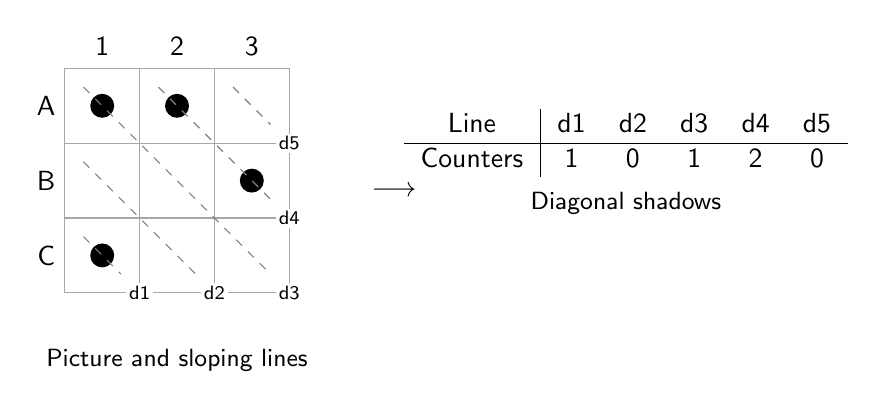
\begin{tikzpicture}[x=0.95cm,y=0.95cm]
\gridbase
\foreach \p in {(0.5,2.5),(1.5,2.5),(2.5,1.5),(0.5,0.5)}\fill \p circle (0.16);
\foreach \x/\y/\u/\v/\d in {0.25/0.75/0.75/0.25/1,0.25/1.75/1.75/0.25/2,0.25/2.75/2.75/0.25/3,1.25/2.75/2.75/1.25/4,2.25/2.75/2.75/2.25/5}{\draw[gray,dashed] (\x,\y)--(\u,\v);\node[fill=white,inner sep=1pt,font=\scriptsize] at (\u+0.25,\v-0.25){d\d};}
\node at (4.4,1.35){$\longrightarrow$};
\node at (7.5,2.0){\begin{tabular}{c|ccccc}Line&d1&d2&d3&d4&d5\\\hline Counters&1&0&1&2&0\end{tabular}};
\node[font=\small] at (1.5,-0.9){Picture and sloping lines};\node[font=\small] at (7.5,1.2){Diagonal shadows};
\end{tikzpicture}
\end{center}
\problem{1}{Place three counters, with one in each row and one in each column. Can two different pictures have the same five diagonal shadows? Find them, or explain why they cannot.}
\vspace{4pt}
\diagboard\hfill\diagboard
\vspace{7pt}
\begin{tabular}{c|p{0.65in}|p{0.65in}|p{0.65in}|p{0.65in}|p{0.65in}}Line&d1&d2&d3&d4&d5\\\hline\rule{0pt}{28pt}Counters&&&&&\end{tabular}
\lines{3}
\newpage
\problem{2}{One player secretly chooses one of the six pictures below and covers every cell of their grid. The guesser names a cell, such as B3; the player says ``occupied'' or ``empty.'' Keep the candidate pictures visible. Naming the determined picture is free. Only a question about a covered cell counts. How few cell questions can you use to identify the hidden picture, even when your opponent chooses the hardest one?}
\begin{center}
\candidate{1}{1,2,3}\hspace{1.2cm}\candidate{2}{1,3,2}\hspace{1.2cm}\candidate{3}{2,1,3}
\par\vspace{14pt}
\candidate{4}{2,3,1}\hspace{1.2cm}\candidate{5}{3,1,2}\hspace{1.2cm}\candidate{6}{3,2,1}
\end{center}
\lines{8}
\newpage
\problem{3}{Use the same six hidden pictures. This time choose every cell question before your opponent answers any of them. What is the fewest questions that always identify the picture? Mark the cells you would ask about and explain why fewer cannot work.}
\vspace{12pt}
\board\hfill\board
\vspace{14pt}
\lines{10}
\newpage
\problem{4}{For each board, place counters to match the row and column counts. If a board cannot be filled, explain why. }
\vspace{8pt}
\marginboard{3,3,0}{3,3,0}\hfill\marginboard{3,2,1}{2,2,2}
\par\vspace{20pt}
\marginboard{2,2,2}{3,3,0}\hfill\marginboard{3,3,1}{3,3,1}
\vspace{12pt}
\lines{3}
\end{document}
